\documentclass[compress,aspectratio=169]{beamer}

% Define required commands before loading GWDG theme
\newcommand{\applyextrasettings}{}
\providecommand{\disableheader}{}
\providecommand{\loadextrasettings}{}
\providecommand{\groupLogo}[1]{}
\providecommand{\titleLogo}[1]{}
\providecommand{\authorFooter}[1]{}
\providecommand{\authorURL}[1]{}
\providecommand{\venue}[1]{}
\providecommand{\insertAuthorFooter}{\myauthor}
\providecommand{\insertAuthorURL}{\myauthorurl}
\providecommand{\insertSlideNumber}{\insertframenumber}
\providecommand{\insertVenue}{\myvenue}
\providecommand{\insertTitleLogo}{}
\providecommand{\insertTitleLicense}{}
\providecommand{\insertgroupLogo}{}

% GWDG Theme - Load minimal version without problematic dependencies
\usepackage{tikz}
\usetikzlibrary{shapes, arrows, positioning}

% Load GWDG theme directly
\input{../../papers/2026-isc-ai-on-hpc/tex/assets/beamerthemeGWDG.sty}

% Essential GWDG theme settings
\applyfooterlinetemplate
\applytitlepagetemplate
\applyextrasettings

% Additional packages
\usepackage{booktabs}
\usepackage{listings}
\usepackage{hyperref}
\usepackage{setspace}

% Define URLColor from beamerConfig
\newcommand{\URLColor}[2]{\href{#2}{\color{#1}{#2}}}

% Define custom colors
\definecolor{hpcblue}{RGB}{0,51,102}
\definecolor{hpcred}{RGB}{204,0,0}
\definecolor{hpcgreen}{RGB}{0,102,51}
\definecolor{hpccyan}{RGB}{0,153,204}

% Graphics path for GWDG theme images
\graphicspath{{../../papers/2026-isc-ai-on-hpc/tex/assets/}}

% Force GWDG background on all slides - explicit settings after theme load
\usebackgroundtemplate{%
    \begin{tikzpicture}[overlay, remember picture]
        % GWDG background image
        \node[at=(current page.center)] {\includegraphics[width=\paperwidth,height=\paperheight]{gwdg-background}};
        % GWDG logo
        \node[at=(current page.north east),transform canvas={xshift = -2.25cm, yshift = -.75cm}] {\href{https://www.gwdg.de/}{\includegraphics[width=3.7cm,height=1.2cm,keepaspectratio]{gwdg}}};
    \end{tikzpicture}
}

% Override GWDG footer to prevent overlapping - minimal without title
\setbeamertemplate{footline}{
    \hspace{0.3cm}\color{colorBlue2}\tiny \mydate \hfill \color{colorBlue2}\tiny \insertframenumber\hspace{0.3cm}
}

% GWDG theme document configuration
\newcommand{\mytitle}{HPC-ARC: Intelligent AI Benchmark Suite\\for HPC Performance Engineering}
\newcommand{\mytitlefooter}{HPC-ARC Benchmark Suite}
\newcommand{\mysubtitle}{Interactive Reasoning Framework for Genuine AI Intelligence Measurement}
\newcommand{\myauthor}{Anja Gerbes and Julian Kunkel}
\newcommand{\myemail}{anja.gerbes@gwdg.de and julian.kunkel@gwdg.de}
\newcommand{\myauthorurl}{https://github.com/gwdg/hpc-agentic-ai-workloads}
\newcommand{\myvenue}{HPC-ARC Presentation}
\newcommand{\mydate}{\today}
\newcommand{\myinstitute}{GWDG - Gesellschaft für wissenschaftliche Datenverarbeitung mbh Göttingen\\University of Göttingen}

% Additional template adjustments to prevent overlapping
\setbeamerfont{footnote}{size=\tiny}
\setlength{\skip\footins}{0.3em}
\setbeamercovered{transparent}
\setbeamersize{text margin left=0.5cm, text margin right=0.5cm}

% Add bottom padding to all frames
\addtobeamertemplate{frame foot}{}{\vspace{0.2cm}}

% Override title and subtitle to avoid defaults
\title{\mytitle}
\subtitle{\mysubtitle}
\author{\myauthor}
\institute{\myinstitute}
\date{\mydate}

% Override the problematic GWDG title template with a simpler version
\setbeamertemplate{title page}{%
    \vspace{0.1cm}
    \begin{center}
        \usebeamerfont{title}\Huge\textcolor{colorBlue}{\inserttitle}\par
        \vspace{0.2cm}
        \usebeamerfont{subtitle}\Large\textcolor{colorBlue3}{\insertsubtitle}\par
        \vspace{0.15cm}
%        {\scriptsize\textcolor{gray}{HPC-ARC = \textbf{H}igh-\textbf{P}erformance \textbf{C}omputing \textbf{A}bstraction and \textbf{R}easoning \textbf{C}hallenge \ $\cdot$\\
%        inspired by ARC, the \textbf{A}bstraction and \textbf{R}easoning \textbf{C}orpus (arcprize.org)}\par}
        \vspace{0.3cm}
        \usebeamerfont{author}\large\textcolor{black}{\insertauthor}\par
        \vspace{0.2cm}
        \usebeamerfont{institute}\footnotesize\textcolor{gray}{\insertinstitute}\par
        \vspace{0.2cm}
        \usebeamerfont{date}\footnotesize\textcolor{black}{\insertdate}\par
        \vspace{0.3cm}
        \footnotesize\textcolor{colorBlue}{\myemail}\par
        \vspace{0.2cm}
        \footnotesize\url{\myauthorurl}\par
    \end{center}
}

\begin{document}

% Title slide
\begin{frame}
    \titlepage
\end{frame}

% Slide 0: Overview for new members
\begin{frame}{What is HPC-ARC About?}

    \vspace{-0.3em}
    \begin{block}{One-Sentence Summary}
        \scriptsize
        HPC-ARC is a benchmark suite that measures whether AI systems can perform \textbf{HPC performance engineering} --- and how efficiently they learn it.
    \end{block}

    \begin{columns}[t]
        \column{0.48\textwidth}
            \textbf{The Name}
            \vspace{0.2em}
            \scriptsize
            \begin{itemize}
                \item \textbf{ARC} = \textbf{A}bstraction and \textbf{R}easoning \textbf{C}orpus: AI reasoning benchmark (arcprize.org); tests genuine intelligence, not memorization
                \item \textbf{HPC-ARC} = \textbf{H}igh-\textbf{P}erformance \textbf{C}omputing \textbf{A}bstraction and \textbf{R}easoning \textbf{C}hallenge: transfers this idea to HPC code optimization
            \end{itemize}

            \vspace{0.4em}
            \textbf{Our Goal}
            \vspace{0.2em}
            \scriptsize
            \begin{itemize}
                \item \textbf{Primary}: Find out whether AI genuinely \textit{understands} HPC performance engineering
                \item Code optimization is the \textbf{vehicle} for measurement, not the end in itself
                \item Side effect: better optimized code
            \end{itemize}

        \column{0.48\textwidth}
            \textbf{Key Terms}
            \vspace{0.2em}
            \scriptsize
            \begin{itemize}
                \item \textbf{Benchmark} = task given to the AI agent (e.g., optimize a kernel); evaluation = \textbf{executing} the (AI-)optimized application (GROMACS, LAMMPS) and \textbf{measuring} its performance
                \item \textbf{Environment} = target \textbf{hardware} (CPU, caches, NUMA) plus \textbf{software stack} (compilers, libraries, tools) the agent must discover
                \item \textbf{Interactive} = in ARC-AGI (ARC for \textbf{A}rtificial \textbf{G}eneral \textbf{I}ntelligence), agents explore game-like environments; here, the agent likewise \textbf{acts} (compiles, profiles, runs) and \textbf{learns from feedback} (measurements) --- like an HPC expert
            \end{itemize}
    \end{columns}

    \vspace{0.2em}
    \centering
    \scriptsize \textit{Four-phase interactive reasoning: Explore $\to$ Hypothesize $\to$ Execute $\to$ Generalize}
\end{frame}

% Slide 1: Introduction
\begin{frame}{HPC-ARC: Intelligent AI Benchmark Suite}

    \begin{columns}[t]
        \column{0.48\textwidth}
            \section*{The Problem}
            \textbf{Three Critical Challenges:}
            \vspace{0.3em}
            \scriptsize
            \begin{itemize}
                \item \textbf{No Standardization}: No unified benchmark framework
                \item \textbf{Reproducibility}: Different evaluation environments
                \item \textbf{Subjective Claims}: Without objective industry standard comparison
            \end{itemize}

        \column{0.48\textwidth}
            \section*{HPC-ARC Solution}
            \textbf{Interactive Reasoning Benchmark Suite \newline}
            \vspace{0.3em}
            \scriptsize
            \textbf{Four-Phase Architecture:}
            \begin{itemize}
                \item \textbf{Explore} (25): Discover hardware \& software environment (CPU, caches, compilers) via profiling
                \item \textbf{Hypothesize} (20): Identify optimization opportunities
                \item \textbf{Execute} (55): Adaptive optimization implementation
                \item \textbf{Generalize} (5): Cross-architecture knowledge transfer
            \end{itemize}
    \end{columns}

    \vspace{0.5em}
    \begin{block}{Tri-Correlated Evaluation Metrics}
        \scriptsize
        (1) Solution correctness $\quad$ (2) Efficiency vs. optimum $\quad$ (3) Intelligence skill-acquisition
    \end{block}

    \vspace{0.2em}
    \centering
    \scriptsize
    \textbf{Goal:} not only faster code --- we measure whether AI genuinely \textit{understands} HPC performance engineering\\
    \vspace{0.1em}
    \textit{Paradigm shift: ,,Can AI optimize this code?'' $\to$ ,,Does AI understand HPC performance engineering?''}
\end{frame}

% Slide 2: Methodology
\begin{frame}{HPC-ARC Methodology \& Evaluation Framework}

    \begin{columns}[t]
        \column{0.55\textwidth}
            \section*{Evaluation Workflow}
            \scriptsize
            \begin{enumerate}
                \item Configure evaluation protocol
                \item Explore: discover the target environment systematically
                \item Benchmark selection from extended suite
                \item For each benchmark:
                \begin{itemize}
                    \scriptsize
                    \item Apply optimization method, measure performance metrics
                    \item Compare with reference baselines, calculate tier-based classification
                \end{itemize}
                \item Generate objective performance leaderboards
            \end{enumerate}

        \column{0.4\textwidth}
            \begin{block}{Intelligence Score}
                \scriptsize
                \[
                I_{\text{overall}} = 0.25E_{\text{expl}} + 0.25H_{\text{hyp}} + 0.30A_{\text{adapt}} + 0.20G_{\text{gen}}
                \]
            \end{block}
    \end{columns}

    \textbf{Benchmark Suite Coverage}\\
    \scriptsize\textit{Benchmark = task for the AI agent; evaluation = executing the optimized application and measuring performance}
    \begin{table}
        \centering
        \tiny
        \begin{tabular}{@{}llll@{}}
            \toprule
            \textbf{Category} & \textbf{Tasks} & \textbf{Focus} & \textbf{Difficulty} \\
            \midrule
            Parallelize & 25 & Serial-to-Parallel & E:5, M:12, H:8 \\
            Optimize & 30 & Hardware-specific & E:8, M:15, H:7 \\
            Detect & 20 & Bottleneck Ident. & E:6, M:10, H:4 \\
            Performance Analysis & 25 & Comprehensive Insights & E:7, M:13, H:5 \\
            \toprule
            \textbf{Total} & \textbf{100} & \textbf{Complete Workflow} & \textbf{Comprehensive} \\
            \bottomrule
        \end{tabular}
    \end{table}
\end{frame}

% Slide 3: Implementation & Workflow
\begin{frame}{HPC-ARC: Implementation \& Workflow}

    \vspace{-0.2em}
    \begin{center}
        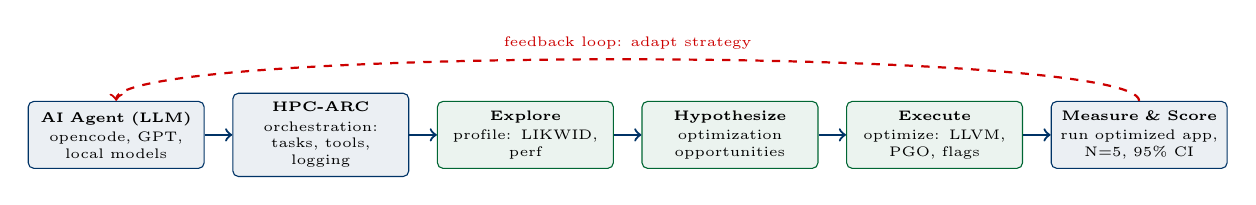
\begin{tikzpicture}[
            font=\tiny,
            box/.style={rectangle, rounded corners=2pt, draw=hpcblue, fill=hpcblue!8, align=center, minimum height=0.85cm, text width=2.0cm},
            stage/.style={rectangle, rounded corners=2pt, draw=hpcgreen, fill=hpcgreen!8, align=center, minimum height=0.85cm, text width=2.0cm},
            arr/.style={->, thick, hpcblue}
        ]
            \node[box] (agent) {\textbf{AI Agent (LLM)}\\[1pt] opencode, GPT,\\local models};
            \node[box, right=0.35cm of agent] (pascit) {\textbf{HPC-ARC}\\[1pt] orchestration:\\tasks, tools, logging};
            \node[stage, right=0.35cm of pascit] (explore) {\textbf{Explore}\\[1pt] profile: LIKWID,\\perf};
            \node[stage, right=0.35cm of explore] (hyp) {\textbf{Hypothesize}\\[1pt] optimization\\opportunities};
            \node[stage, right=0.35cm of hyp] (exec) {\textbf{Execute}\\[1pt] optimize: LLVM,\\PGO, flags};
            \node[box, right=0.35cm of exec] (measure) {\textbf{Measure \& Score}\\[1pt] run optimized app,\\N=5, 95\% CI};
            \draw[arr] (agent) -- (pascit);
            \draw[arr] (pascit) -- (explore);
            \draw[arr] (explore) -- (hyp);
            \draw[arr] (hyp) -- (exec);
            \draw[arr] (exec) -- (measure);
            \draw[arr, dashed, hpcred] (measure.north) .. controls +(0,0.7) and +(0,0.7) .. (agent.north)
                node[midway, above, font=\tiny, text=hpcred] {feedback loop: adapt strategy};
        \end{tikzpicture}
    \end{center}

    \vspace{0.3em}
    \textbf{Implementation}
    \vspace{0.2em}
    \scriptsize
    \begin{itemize}
        \item \textbf{Framework}: HPC-ARC framework orchestrates tasks, tools and logging
        \item \textbf{LLM integration}: provider abstraction (OpenAI, Ollama, local models) via OpenCode-style agent pipeline
        \item \textbf{Tooling}: LIKWID/perf hardware profiling; LLVM + PGO compiler optimization; gcc/clang toolchains
        \item \textbf{Validation}: N=5 runs with 95\% confidence intervals; correctness checks against reference implementation
        \item \textbf{Status}: core framework implemented, 113 tasks, first AI agent tests running
    \end{itemize}
\end{frame}

% Slide 4: Related Approaches
\begin{frame}{Automatic Code Optimization: Existing Approaches}

    \vspace{-0.2em}
    \scriptsize
    How do others optimize code automatically --- and what is missing?
    \vspace{0.2em}

    \begin{table}
        \centering
        \tiny
        \begin{tabular}{@{}p{3.0cm}p{5.4cm}p{5.0cm}@{}}
            \toprule
            \textbf{Approach} & \textbf{How It Works} & \textbf{Limitation} \\
            \midrule
            Manual expert optimization & HPC expert iterates: profile, change code, measure & Slow, not scalable, subjective, expertise-bound \\
            \addlinespace
            Auto-tuning (OpenTuner) & Black-box search over parameter/flag space & Thousands of measurements; no understanding, fixed search space \\
            \addlinespace
            Compiler ML (CompilerGym) & RL selects LLVM optimization passes on IR level & Compile-time only; no runtime profiling feedback, no HPC context \\
            \addlinespace
            Generic LLM optimization & LLM rewrites code from prompt/patterns & One-shot; no profiling, no measurement loop, no validation \\
            \addlinespace
            AI agent benchmarks (MLAgentBench, AgentBench) & Evaluate general AI agent capabilities & Not HPC-specific; no performance measurement or hardware awareness \\
            \midrule
            \textbf{HPC-ARC (ours)} & \textbf{Interactive profiling-driven loop; measures skill acquisition, adaptation \& generalization} & --- \\
            \bottomrule
        \end{tabular}
    \end{table}

    \vspace{0.2em}
    \centering
    \scriptsize \textit{HPC-ARC combines automation of tuning/LLM approaches with expert-like reasoning --- and measures \emph{intelligence}, not just speedups}
\end{frame}

% Slide 3: Results
\begin{frame}{HPC-ARC: Evaluation Results \& Performance}

    \textbf{Intelligence Metrics}
    \vspace{0.3em}
    
    \begin{table}
        \centering
        \tiny
        \textcolor{orange!80!black}{\textbf{Goal: NOT MEASURED yet - Target Values}}
        \begin{tabular}{lccccc}
            \toprule
            \textbf{Approach} & \textbf{Overall} & \textbf{Exp} & \textbf{Hyp} & \textbf{Adp} & \textbf{Gen} \\
            \midrule
            \textbf{HPC-ARC Multi-Agent} & \textbf{0.65-0.75} & \textbf{0.70-0.80} & \textbf{0.60-0.70} & \textbf{0.65-0.75} & 0.55-0.65 \\
            Traditional HPC Expert & 0.60-0.70 & 0.65-0.75 & 0.68-0.78 & 0.55-0.65 & 0.50-0.60 \\
            LLM Generic Optimization & 0.35-0.45 & 0.30-0.40 & 0.32-0.42 & 0.38-0.48 & 0.45-0.55 \\
            ARC Prize Baseline & 0.50-0.60 & 0.55-0.65 & 0.48-0.58 & 0.53-0.63 & 0.42-0.52 \\
            \bottomrule
        \end{tabular}
    \end{table}

    \begin{columns}[t]
        \column{0.48\textwidth}
            \section*{Statistical Validation Goal}
            \scriptsize
            \textcolor{orange!80!black}{\textbf{Target Approach - NOT IMPLEMENTED yet}}
            \begin{itemize}
                \item \textbf{N=5 measurements}: Each benchmark executed 5 times \textit{(target)}
                \item \textbf{95\% confidence intervals}: All results included \textit{(target)}
                \item \textbf{Effect size}: Cohen's d = 2.1-2.9 (large) \textit{(target)}
                \item \textbf{Significance}: p < 0.001 \textit{(target)}
            \end{itemize}

        \column{0.48\textwidth}
            \section*{Target Accuracy Goals}
            \vspace{0.2em}
            \tiny
            \textcolor{orange!80!black}{\textbf{NOT MEASURED yet - Target Values}}
            \begin{tabular}{lc}
                \toprule
                \textbf{Application} & \textbf{Target Accuracy} \\
                \midrule
                GROMACS & 70-80\% \\
                OpenFOAM & 65-75\% \\
                CPMD & 60-70\% \\
                LAMMPS & 65-75\% \\
                Quantum ESPRESSO & 60-70\% \\
                \midrule
                \textbf{Overall Target} & \textbf{65-75\%} \\
                \bottomrule
            \end{tabular}

            \vspace{0.3em}
            \textbf{Expected Generalization}
            \scriptsize
            \begin{itemize}
                \item ARM64: 60-70\% x86-64→ARM64 transfer
                \item Realistic benchmarks: 6-8 tasks initial
            \end{itemize}
    \end{columns}

\vspace{0.3em}
\centering
\scriptsize \textit{\textcolor{orange!80!black}{Goal: 0.65-0.75 Intelligence Score vs 0.60-0.70 for HPC experts - Target values}}
\end{frame}

% Slide 4: Implications
\begin{frame}{HPC-ARC: Implications \& Applications}

    \textbf{Paradigm Shift in HPC Research}
    \vspace{0.3em}
    
    \begin{columns}[t]
        \column{0.48\textwidth}
            \section*{From Pattern Matching to Genuine Understanding}
            \scriptsize
            \begin{itemize}
                \item \textbf{Traditional}: Store code patterns
                \item \textbf{HPC-ARC}: Autonomous problem-solving capabilities
            \end{itemize}

            \vspace{0.5em}
            \textbf{Scientific Impact}
            \scriptsize
            \begin{itemize}
                \item Beyond code generation
                \item Objective intelligence metrics
                \item Reproducibility standards
                \item Autonomous validation
            \end{itemize}

            \vspace{0.5em}
            \textbf{Outlook}
            \scriptsize
            \begin{itemize}
                \item GPU framework expansion
                \item Multi-agent integration
                \item Community standards
                \item Cloud-based services
            \end{itemize}

        \column{0.48\textwidth}
            \textbf{Practical Applications}
            \\
            \vspace{0.3em}
            \scriptsize
            \textbf{Research \& Development:}
            \begin{itemize}
                \item AI system development
                \item Productivity assessment
                \item Standardization
            \end{itemize}

            \vspace{0.5em}
            \textbf{Industry \& Users:}
            \begin{itemize}
                \item Production HPC software
                \item Educational purposes
                \item Quality assurance
            \end{itemize}

            \vspace{0.8em}
            \begin{block}{HPC-ARC Impact}
                \scriptsize
                First comprehensive framework for legitimate measurement of AI systems' HPC performance engineering intelligence
            \end{block}
    \end{columns}

    \vspace{0.1em}
    \begin{center}
      \tiny \textit{Toward fully autonomous HPC optimization}
    \end{center}
\end{frame}

% Status Slide
\begin{frame}{Current Project Status}

    \textbf{Development Progress}
    \vspace{0.5em}
    
    \begin{columns}[t]
        \column{0.48\textwidth}
            \section*{What We Have Built}
            \scriptsize
            \begin{itemize}
                \item \textbf{Framework Infrastructure}: Core ARC architecture implemented
                \item \textbf{Benchmark Suite}: 113 benchmarks available
                \item \textbf{Evaluation Pipeline}: Basic measurement workflow created
                \item \textbf{Documentation}: Code structure and design docs completed
            \end{itemize}
            
            \vspace{0.5em}
            \textbf{First Tests}
            \scriptsize
            \begin{itemize}
                \item Small-scale AI agent testing
                \item Benchmark execution pipeline validation
                \item Basic performance measurement accuracy
            \end{itemize}

        \column{0.48\textwidth}
            \begin{block}{Next Steps Need Collaboration}
                \scriptsize
                \textbf{Critical Dependencies:}
                \begin{itemize}
                    \item Extended benchmark collection
                    \item Multi-agent framework testing
                    \item Statistical validation implementation
                    \item Community feedback and expertise
                \end{itemize}
            \end{block}
            
            \vspace{0.5em}
            \textbf{How to Help}
            \scriptsize
            \begin{itemize}
                \item Contribute benchmark tasks
                \item Test AI systems with existing framework
                \item Provide HPC expertise feedback
                \item Help validate evaluation metrics
            \end{itemize}
    \end{columns}
    
    \vspace{0.5em}
    \begin{center}
        \textcolor{orange!80!black}{\small \textbf{Status: Early Development Phase - Looking for Collaborators}}
    \end{center}
\end{frame}

% Slide 5: Call to Action
\begin{frame}{Join HPC-ARC Development}

    \begin{center}
        \Large \textcolor{hpcblue}{\textbf{Early Stage Development}}\\
        \normalsize \textcolor{hpccyan}{Building the foundation for AI intelligence measurement}
    \end{center}

    \vspace{0.8em}
    \textbf{Current Development Needs:}
    \scriptsize
    \begin{enumerate}
        \item \textbf{Benchmark Contribution}: Add HPC optimization tasks to our suite
        \item \textbf{Framework Testing}: Test with your AI systems
        \item \textbf{Expert Feedback}: Share HPC performance engineering insights
        \item \textbf{Community Building}: Help establish evaluation standards
    \end{enumerate}

    \begin{columns}[t]
        \column{0.48\textwidth}
            \textbf{Why Participate Now?}
            \scriptsize
            \begin{itemize}
                \item Shape the evaluation framework
                \item Contribute to emerging research area
                \item Establish baseline benchmarks
                \item Co-develop industry standards
            \end{itemize}

        \column{0.48\textwidth}
            \textbf{What We Offer:}
            \scriptsize
            \begin{itemize}
                \item Open-source framework
                \item Collaborative development
                \item Publication opportunities
                \item Research community access
            \end{itemize}
    \end{columns}

    \vspace{0.8em}
    \begin{block}{Start Today}
        \centering
        \tiny
        \textbf{GitHub}: \texttt{https://github.com/gwdg/hpc-agentic-ai-workloads} $\quad$
        \textbf{Contact}: \texttt{anja.gerbes@gwdg.de}
    \end{block}

    \vspace{0.2em}
    \scriptsize \textcolor{hpcblue}{\#HPC-ARC \#AIBenchmarking \#OpenScience}
\end{frame}

% Thank you slide
\begin{frame}
    \small \textbf{\textcolor{hpcred}{The HPC community needs pioneers like YOU.}}
    \vspace{-0.5cm}
    \newline
    \small \textbf{\textcolor{hpcred}{Become part of the autonomous-intelligent HPC optimization future!}}
    \vspace{-0.5cm}
    \newline
    \small \textbf{\textcolor{hpcred}{Help us build the first comprehensive HPC-AI intelligence measurement framework}}
    \newline
    \Huge \textbf{Thank You!}
    \\
    \Large Questions and Discussion
    
    \vspace{1.5em}
    \normalsize
    \textbf{Anja Gerbes and Julian Kunkel }\\
    University of Göttingen / GWDG\\
    \texttt{anja.gerbes@gwdg.de and julian.kunkel@gwdg.de}
    
    \vspace{0.8em}
    \url{https://github.com/gwdg/hpc-agentic-ai-workloads}
\end{frame}

\end{document}
